%% ============================================================
%% main.tex — Conflict-Gated Arbitration for Infrared–Visible
%% Image Fusion (Springer sn-jnl, sn-mathphys-num references)
%%
%% Assembled by formatter_agent (Phase 7, 2026-09-14) from
%% writing/00-abstract.md, 01, 02, 04, 05, 06; bibliography from
%% writing/07-references.md (citation-check, dispositions applied).
%% Preamble mirrors the official sn-article.tex v3.1 template.
%% ============================================================

\documentclass[pdflatex,sn-mathphys-num]{sn-jnl}

%%%% Standard Packages
\usepackage{graphicx}%
\usepackage{multirow}%
\usepackage{amsmath,amssymb,amsfonts}%
\usepackage{amsthm}%
\usepackage{mathrsfs}%
\usepackage[title]{appendix}%
\usepackage{xcolor}%
\usepackage{textcomp}%
\usepackage{manyfoot}%
\usepackage{booktabs}%
\usepackage{algorithm}%
\usepackage{algorithmicx}%
\usepackage{algpseudocode}%
\usepackage{listings}%

%% as per the requirement new theorem styles can be included as shown below
\theoremstyle{thmstyleone}%
\newtheorem{theorem}{Theorem}%
\newtheorem{proposition}[theorem]{Proposition}%

\theoremstyle{thmstyletwo}%
\newtheorem{example}{Example}%
\newtheorem{remark}{Remark}%

\theoremstyle{thmstylethree}%
\newtheorem{definition}{Definition}%

\raggedbottom

\begin{document}

\title[Conflict-Gated Arbitration for Infrared--Visible Image Fusion]{Conflict-Gated Arbitration for Infrared--Visible Image Fusion}

\author*[1]{\fnm{Author} \sur{Name}}\email{author.name@example.org}

\affil*[1]{\orgdiv{Department}, \orgname{Organization}, \orgaddress{\street{Street}, \city{City}, \postcode{000000}, \country{Country}}}

%%--------------------------------------------
%% Abstract (verbatim from writing/00-abstract.md, English abstract)
%%--------------------------------------------
\abstract{At pixels where infrared and visible images disagree, mainstream fusion networks resolve the conflict by blending --- weighted averaging in feature space --- and any blend cancels the structure that committing to the salient modality would preserve. For visual perception systems that fuse to detect, the objects lost in this cancellation matter. This paper first shows, through a pre-registered, same-budget falsification on the selective state-space backbone S4Fusion, that the prevailing alternative does not fix this: feature-space modulation of the state dynamics, motivated by state-capacity dilution, does not improve structural fusion quality under matched training budget. The residual failure lies outside the state, in the absence of an arbitration decision. We therefore introduce Conflict-Gated Arbitration (CGA), which detects per-pixel cross-modal conflict from image gradients and applies a learned, zero-initialized, image-space per-pixel commitment toward the locally salient modality, acting only where the modalities conflict, so that loading the official checkpoint reproduces the baseline exactly. Across three seeds, the primary criterion replicates: gains on high-conflict object recall are statistically significant yet below the stricter pre-registered thresholds, and significant structural costs in SF and AG accompany them. On full-reference quality the method attains the leading QABF among the eight unified-evaluation baselines and a statistical tie on VIF, though SF and MI remain below the official released weights. All numbers come from one frozen evaluation; training-free pre-checks, mechanism visualizations and a registered distillation failure are reported alongside the gains. Code and protocols are released for full reproduction.}

\keywords{infrared--visible image fusion, conflict arbitration, selective state-space models, zero-initialized gating, object detection, image quality assessment}

\maketitle

%%=============================================================
%% §1 Introduction
%% Source: writing/01-intro-mechanism.md — Draft paragraphs,
%% "Why S4Fusion as the testbed" items, and "Deliberately not
%% claimed" paragraph; process material (outline, claim–evidence
%% map, assumptions) omitted per assembly rules.
%%=============================================================
\section{Introduction}\label{sec:intro}

Selective state-space models (SSMs) have recently become the backbone of infrared--visible image fusion because their linear-time global receptive field scales better than self-attention on large inputs \cite{ma2025s4fusion,gu2023mamba}. Yet their usefulness at high resolution is constrained by a fundamental capacity problem: the recurrent state has bounded capacity, and long sequences dilute the information each state slot can retain --- when the contextual information exceeds the state capacity, the model even fails to learn what to forget \cite{chen2025stuffed}; the state transition is further controlled by the spectral properties of the decay matrix, so that poorly managed states drift or vanish over long horizons \cite{lu2025mambamodulation,ali2025hidden}. This motivated us to hypothesize that fusion failures at high resolution originate \emph{inside} the SSM state dynamics --- specifically, that injecting per-pixel boundary reliability into the selective parameters $B$, $C$ and $\Delta$ would re-allocate state capacity toward modality boundaries where cross-modal conflict is largest.

We tested this hypothesis under strictly controlled conditions: every configuration was fine-tuned from the same public S4Fusion weights with identical budget (crop 128, 20 epochs, seed 42, same data), and evaluated with the same overlap-tiled inference protocol (native resolution with replicate padding where tile sizes require it) on M3FD \cite{liu2022tardal}. The result was a falsification. Relative to the same-budget baseline, the state-modulated model significantly \emph{degraded} structural metrics (SF $-0.019$, AG $-0.013$, QABF $-0.0005$, Holm-corrected $p < 0.05$). Feature-space modulation of SSM dynamics, despite its theoretical appeal, does not, under this registered parameterization, yield structural fusion gains; the residual failure is located outside the state.

The failure is instead in the arbitration decision. Where the two modalities disagree --- opposite edge orientation or polarity at the same pixel --- any \emph{blend} (weighted average in image or feature space) cancels structure, whereas \emph{committing} to the locally salient modality preserves it. We verified this in a training-free pre-check on M3FD detection: committing toward the max-response modality in conflict regions recovers objects that blending loses. We therefore introduce \textbf{Conflict-Gated Arbitration (CGA)}, which (i)~detects per-pixel modal conflict from image gradients, (ii)~learns a per-pixel commitment toward the salient modality, and (iii)~applies it \emph{only in conflict regions} through a zero-initialized gate, so that loading the official S4Fusion checkpoint reproduces the baseline exactly and the design is compatible with prior weights \cite{bachlechner2021rezero}. Beyond avoiding the artifact tax of global blending, CGA localizes intervention to the pixels where a decision is genuinely required --- a qualitatively different mechanism from feature-space modulation, and one that directly targets the objects downstream detection systems lose.

S4Fusion serves as the testbed for three reasons. First, it is a representative of the scan-and-blend operator class: the question this paper asks --- \emph{does feature-space modulation of SSM state dynamics fix fusion at boundaries?} --- is a question about an operator class (linear-time scan backbones that mix modal representations), not about one model, and S4Fusion \cite{ma2025s4fusion} is the representative open, published scan-and-blend SSM fusion backbone; the (negative) answer obtained on it is informative about the class, and we scope class-level claims to what a single-backbone falsification can support (Section~\ref{sec:limitations}), while it additionally anchors the SSM row of the unified-protocol comparison of Section~\ref{sec:exp}. Second, a public checkpoint is what makes the falsification \emph{controlled}: because official weights are released, every arm of every ablation (same-budget retrain, B/C/$\Delta$ modulation, CGA) fine-tunes from the same starting point under the arm-specific registered schedules disclosed in Section~\ref{sec:exp}, so any metric delta is attributable to the intervention, not to initialization or training-set differences. Third, zero-initialized compatibility validates the arbitration layer \emph{against} the weights it modifies: CGA's gate starts at $\tanh(0)=0$, so loading the official checkpoint reproduces the baseline output exactly, and the trained gate then saturates (frozen visualization record in Section~\ref{sec:exp}), showing that the mechanism is genuinely learned rather than left off.

\emph{Deliberately not claimed}: that S4Fusion is the best fusion model (the frozen comparison table shows EMMA \cite{zhao2024equivariant} leading SF and AG and Diff-IF \cite{yi2024diffif} leading MI --- reported as-is); or that the choice was mechanistically privileged. Across three seeds, the high-conflict recall gain is significant on all three seeds (exact binomial $p = 4.88\times 10^{-4}$ / $4.34\times 10^{-3}$ / $4.34\times 10^{-3}$) yet below the stricter pre-registered thresholds ($+0.02$ recall / mAP50 $+0.01$); SF/AG structural non-inferiority passes on $2/3$ seeds, with seed 42 the borderline exception ($-1.00\%$).

%%=============================================================
%% §2 Related work
%% Source: writing/02-related-work.md — six family sections;
%% classification map converted to transitional prose
%% (journal style); Notes section omitted.
%%=============================================================
\section{Related work}\label{sec:related}

\paragraph{CNN-based fusion.}
Early fusion networks build on autoencoder and dense designs --- DenseFuse \cite{li2019densefuse} with its DenseNet encoder and the unified dense architecture FusionDN \cite{xu2020fusiondn} --- and the adversarial formulation FusionGAN \cite{ma2019fusiongan} made fusion a pixel-level generation game; these lines were later unified under an unsupervised, application-agnostic training scheme in U2Fusion \cite{xu2022u2fusion}. These models achieve strong local structure preservation, but their receptive fields grow only with depth; at modality boundaries the network is forced to resolve conflict by local averaging (or by a discriminator's blending preference), and global structural consistency is achieved (if at all) by stacking layers or scales rather than by an explicit decision about which modality to trust. This is the technical reason CNN fusion degrades in global consistency: the operator has no mechanism to \emph{prefer} one modality at a conflicting pixel; it can only mix local statistics.

\paragraph{Transformer-based fusion.}
Self-attention brought global context to fusion: CDDFuse \cite{zhao2023cddfuse} decomposes common and modality-specific features with correlation-driven branches and restores them with a Transformer; task-driven and meta-learning formulations such as MetaFusion \cite{zhao2023metafusion} adapt fusion to downstream tasks; EMMA \cite{zhao2024equivariant} adds equivariant self-supervision. Attention computes a weighted \emph{average} over all tokens, so a conflicting boundary pixel receives a blend of both modalities' evidence; moreover, quadratic complexity in token count makes full-resolution global attention expensive exactly in the high-resolution regime we target. Decomposition helps, but the output is still a weighted sum --- no commitment is ever made.

\paragraph{Diffusion-based fusion.}
Diffusion models formulate fusion as iterative denoising toward a joint distribution, e.g., DDFM \cite{zhao2023ddfm} and Diff-IF \cite{yi2024diffif}. They capture strong global priors and are robust to modality mismatch, but the generative process \emph{averages} modality evidence under the prior at every step --- there is no mechanism to hard-commit to one modality where they disagree --- and sampling cost (dozens of steps) conflicts with the deployment-efficiency goal. Their global consistency is therefore strong but slow and still non-committal at conflict pixels.

\paragraph{Mamba/SSM-based fusion.}
Selective state spaces entered infrared--visible image fusion nearly simultaneously from several directions: S4Fusion \cite{ma2025s4fusion} applies them with saliency-aware selection, the wavelet-domain W-Mamba \cite{zhang2025wmamba} and the multi-modal FusionMamba \cite{xie2024fusionmamba} (first published online in 2024) appeared in the same window. These inherit linear-time global context from the SSM family \cite{gu2023mamba,dao2024transformers}. The technical limitation is state capacity: recent analyses show that the recurrent state, when overloaded by long sequences, loses its ability to manage what it retains \cite{chen2025stuffed}, and that only the A/$\Delta$ parameters control history decay \cite{ali2025hidden,lu2025mambamodulation}. SSM fusion thus has global context but a bounded, dilutable state --- and, like all scan-based operators, it \emph{scans and blends} rather than deciding. The 2026 wave continues to modify \emph{scan topology} rather than the decision: spatial-frequency interactive scanning \cite{zhu2026interactive}, random shuffle scanning \cite{cao2026shuffle}, and self-supervised consensus among experts \cite{wang2026selfsupervised} --- all of which reorganize \emph{where the scan looks}, not \emph{what the state should commit to} at a conflicting pixel. Our own controlled ablation (Section~\ref{sec:methods}, the feature-space state-modulation hypothesis) shows that, under the registered parameterization, modulating the state dynamics ($B/C/\Delta$) with boundary reliability does \emph{not} improve structural metrics --- the residual failure is the absence of an arbitration decision, which we target instead.

\paragraph{Semantic- and task-guided fusion.}
Task-awareness improves fusion for downstream perception: SeAFusion \cite{tang2022seafusion} distills semantic information into fusion; SegMiF / M2Fusion \cite{liu2023segmif} couple segmentation with fusion; MetaFusion \cite{zhao2023metafusion} adapts via meta-learning; KD-based lightweight variants exist \cite{zhao2023lightweight,wang2025semantic}. These methods guide \emph{where} to look (task semantics) but still resolve conflicting pixels by weighting features; they improve target recall but do not solve the decision problem, and their semantic branches need task labels/extra networks at inference.

\paragraph{Boundary-aware, uncertainty-guided, and conflict-aware fusion.}
Boundary and uncertainty cues are an active, growing direction: boundary-aware uncertainty fusion for medical segmentation (BUFNet \cite{zhou2026bufnet}); boundary-region selective scanning for shadow removal (ShadowMamba \cite{zhu2026shadowmamba}); edge-prior-guided IVIF \cite{yuan2025segment}; edge-guided dual attention \cite{zou2023lightweight}; uncertainty-aware cross-modal fusion for detection \cite{zhao2024uncertainty}. Closest to our setting, ARC3Fusion \cite{tian2026adaptive} explicitly models consensus--complementarity--\emph{conflict} in IVIF --- its conflict estimation even includes edge-strength and orientation mismatch --- and GatedFusion-Net \cite{brenner2026gatedfusion} computes per-pixel modality weights. These confirm that conflict and per-pixel weighting are recognized concerns, yet both operate as \emph{continuous, feature-space soft coordination}: ARC3Fusion routes verified residuals in feature space with a shared encoder, fusing them through per-position three-branch Softmax weights that sum to one, and GatedFusion-Net learns per-pixel Sigmoid confidence masks that gate the thermal and ultraviolet streams additively onto its RGB+DIN base for semantic segmentation. Image-space per-pixel \emph{hard} selection has a long but separate lineage: the classical select/choose fusion rules \cite{burt1993enhanced,zhang1999categorization,piella2003general} formalized ``choose the salient source where they disagree'' for pyramid fusion, and the learning-based multi-focus decision-map line \cite{ma2021endtoend} still makes per-pixel binary decisions --- but driven by defocus in \emph{same-modality} pairs, unrelated to cross-modal conflict. Learned \emph{discrete} routing has also entered IVIF: a concurrent preprint \cite{ma2026dynamic} selects, per pixel, among copy-infrared, copy-visible, and attention-fusion experts via a Gumbel-Softmax straight-through estimator --- the closest existing instance of per-pixel hard choice in cross-modal fusion, yet it operates on invertible-network-decoupled feature components (feature space, not image space), and its routing signal is learned informativeness rather than cross-modal gradient conflict. To the best of our knowledge, no prior IVIF method converts cross-modal gradient-orientation/polarity conflict into a learned, image-space, per-pixel hard-commitment arbitration. Our distinction is therefore positional, not incremental: existing conflict modeling is feature-space and soft; existing discrete routing is feature-space and conflict-agnostic; existing hard selection is same-modality and defocus-driven; we are the first to place a learned hard commitment at cross-modal conflict pixels in image space --- through a zero-initialized gate that preserves the official S4Fusion checkpoint exactly at load time.

%%=============================================================
%% §3 Methods
%% Source: writing/04-methods.md — five subsections;
%% [PENDING-NOT-FROZEN] placeholders converted to LaTeX
%% comments with qualitative in-text wording.
%%=============================================================
\section{Methods}\label{sec:methods}

\subsection{Problem formulation and design requirements}\label{sec:methods:problem}

Let $I_{\mathrm{ir}}, I_{\mathrm{vi}} \in [0,1]^{1\times H\times W}$ be a registered infrared--visible pair, the visible image reduced to its luminance (Y) channel. The backbone, S4Fusion \cite{ma2025s4fusion}, encodes both modalities with selective state-space (SSM) encoders, fuses them at multiple scales in bidirectional-scan fusion blocks, and decodes a fused luminance image $Y = f_\theta(I_{\mathrm{ir}}, I_{\mathrm{vi}})$. The question this section formalizes is where, in such a pipeline, the decision should be made when the two modalities disagree about the same physical structure.

We define cross-modal conflict at a pixel as the conjunction of two conditions: both modalities carry structure there (both gradient magnitudes non-negligible) and their gradient vectors disagree in orientation or polarity --- the common case at modality boundaries, where a thermal edge and its visible counterpart often have opposite polarity. In this regime every convex blend is structurally destructive. If locally $\nabla I_{\mathrm{vi}} \approx -\nabla I_{\mathrm{ir}}$ with common magnitude $g$, the blend $F = w\,I_{\mathrm{ir}} + (1-w)\,I_{\mathrm{vi}}$ with $w \in [0,1]$ has gradient magnitude $|\nabla F| \approx |2w-1|\,g$: it cancels the structure completely at $w = 1/2$ and preserves it only at the endpoints $w \in \{0,1\}$ --- that is, only under full commitment to one modality. A soft weighting, in image space or in feature space, cannot preserve a conflicting boundary; it can only choose how much of it to cancel. A per-pixel weight field is also the wrong instrument for a second reason: optimized over the whole image, it has no pressure to saturate exactly at the pixels where blending fails.

The natural alternative --- giving the operator more capacity to represent boundaries --- we tested directly and rejected: a pre-registered, same-budget falsification (the feature-space arm of Section~\ref{sec:methods:design}) showed that modulating the SSM state dynamics (the $B$, $C$, $\Delta$ parameters) with a learned boundary-reliability map does not improve structural fusion metrics (frozen verdict in Section~\ref{sec:exp}). Under this registered parameterization, the state-capacity dilution account does not transfer to structural gains --- the residual failure is located outside the state, in the absence of an arbitration decision at conflicting pixels.

These observations induce three design requirements. (R1)~\emph{Image-space operation}: which modality to keep at a pixel is defined and observable in image space, and after the falsification above there is no evidence that intervening in feature space transfers to structural gains; image-space operation also leaves the backbone's internals untouched. (R2)~\emph{Conflict-triggered selectivity}: the mechanism must act only where the modalities actually conflict, so non-conflict pixels retain the pretrained model's behaviour exactly and any measured gain is attributable to arbitration rather than to a global perturbation. (R3)~\emph{Per-pixel commitment behind a zero-initialized gate}: at a conflict pixel the output should move toward the locally salient modality rather than a blend of both, and the whole mechanism must start as an exact identity so that pretrained weights --- including the official public checkpoint --- remain valid. We refer to the resulting mechanism class as image-space per-pixel commitment at conflict pixels: an arbitration added on top of a fusion backbone, not a re-weighting inside it.

\subsection{Conflict-Gated Arbitration}\label{sec:methods:cga}

Conflict-Gated Arbitration (CGA) implements the three requirements as one image-space module: detect conflict, form a per-pixel commitment toward the salient modality, and apply that commitment through a zero-initialized gate only in conflict regions. It is attached once, at the output of the S4Fusion decoder: the augmented forward pass retains the original inputs at native resolution and applies CGA to $(I_{\mathrm{ir}}, I_{\mathrm{vi}}, Y)$, returning the arbitrated image $F$; encoders, fusion blocks and decoder are untouched, and the interface (two source images plus a fused image) is backbone-agnostic in principle.

\paragraph{Conflict signal.}
For each modality $m \in \{\mathrm{ir}, \mathrm{vi}\}$, fixed $3\times 3$ Sobel kernels scaled by $1/4$ give gradient components $G_x^m, G_y^m$ and magnitude
\begin{equation}\label{eq:gm}
g_m = \sqrt{(G_x^m)^2 + (G_y^m)^2 + \varepsilon}, \qquad \varepsilon = 10^{-6},
\end{equation}
and orientation agreement between the two gradient fields is their cosine
\begin{equation}\label{eq:cos}
c = \frac{G_x^{\mathrm{ir}} G_x^{\mathrm{vi}} + G_y^{\mathrm{ir}} G_y^{\mathrm{vi}}}{g_{\mathrm{ir}}\, g_{\mathrm{vi}} + \varepsilon} \in [-1, 1].
\end{equation}
The conflict prior is the closed form
\begin{equation}\label{eq:kappa}
\kappa = \min\!\left(g_{\mathrm{ir}}, g_{\mathrm{vi}}\right)\, \frac{1 - c}{2}.
\end{equation}
The minimum makes the signal symmetric: conflict requires structure in \emph{both} modalities --- a pixel where only one modality has an edge contributes exactly zero --- while $(1-c)/2$ maps aligned gradients ($c \approx 1$) to $\kappa \approx 0$ and opposite polarity ($c \approx -1$) to its maximum. The prior is computed in fp32 even under mixed precision, so that the square-root epsilon remains effective, and is normalized per image by its spatial maximum and clipped, $\hat\kappa = \mathrm{clip}\big(\kappa / (\max_u \kappa + \epsilon);\, 0, 1\big)$, serving as a self-supervised target below. No annotation enters any of these expressions; the signal is derived from the input pair alone.

\paragraph{Learned conflict map.}
The prior is pointwise and fixed; the mechanism learns its conflict map from richer evidence. A convolutional head $h_c$ (a $3\times 3$ convolution from 5 to 16 channels, SiLU, a depthwise $3\times 3$ convolution, SiLU, a $1\times 1$ convolution to one channel) receives the stack $[I_{\mathrm{ir}}, I_{\mathrm{vi}}, g_{\mathrm{ir}}, g_{\mathrm{vi}}, \hat\kappa]$ and produces
\begin{equation}\label{eq:M}
M = \sigma\big(h_c([I_{\mathrm{ir}}, I_{\mathrm{vi}}, g_{\mathrm{ir}}, g_{\mathrm{vi}}, \hat\kappa])\big) \in [0,1]^{1\times H\times W},
\end{equation}
a map that can absorb context the pointwise prior cannot --- textured versus structural disagreement, for instance --- while remaining grounded on $\hat\kappa$ through the loss below.

\paragraph{Commit selection.}
The commitment is a per-pixel convex selection between the two source images,
\begin{equation}\label{eq:commit}
K = s\, I_{\mathrm{ir}} + (1-s)\, I_{\mathrm{vi}}, \qquad s = \sigma\big(h_s([I_{\mathrm{ir}}, I_{\mathrm{vi}}, g_{\mathrm{ir}}, g_{\mathrm{vi}}]) + 2p\big),
\end{equation}
where $h_s$ is a $3\times 3$ convolution (4 to 16 channels), SiLU, $1\times 1$ convolution stack and $p = 2\cdot\mathbb{1}[g_{\mathrm{ir}} > g_{\mathrm{vi}}] - 1 \in \{-1, +1\}$ names the modality with the larger local gradient. The final layer of $h_s$ is initialized to zero, so before training the selection reduces to $s = \sigma(2p) \approx 0.88$ toward that modality --- the max-response commit identified by the training-free pre-check reported in the Introduction --- and training may sharpen or override it.

\paragraph{Gate and combination.}
A single scalar $\alpha$, zero-initialized, bounds the mechanism globally; the learned conflict map localizes it:
\begin{equation}\label{eq:gate}
w = \tanh(\alpha)\cdot M, \qquad F = Y + w \odot (K - Y),
\end{equation}
equivalently $F = (1-w) \odot Y + w \odot K$ with per-pixel $w \in [0, \tanh\alpha]$. Where $M \to 0$ the output equals the backbone's fusion $Y$ exactly; at conflict pixels it moves toward the commitment by at most $\tanh(\alpha)$. At initialization $\tanh(0) = 0$, hence $F \equiv Y$ at every pixel: the module is an exact identity before training.

\paragraph{Training objective.}
The backbone keeps the repository's standard fine-tuning objective --- an intensity term ($\mathcal{L}_1$ to the pixelwise maximum of the inputs), a gradient term ($\mathcal{L}_1$ to the pixelwise maximum of the Sobel magnitudes), an edge-aware smoothness term, and a cross-resolution scale-consistency term --- at repository defaults. CGA adds two terms. The conflict grounding term is a binary cross-entropy with logits between the head's logit and the detached target $\hat\kappa$ (numerically safe under mixed precision). The conflict-gated commit term is
\begin{equation}\label{eq:commitloss}
\mathcal{L}_{\mathrm{commit}} = \frac{1}{HW}\sum_{u} \bar{M}(u)\,\big(F(u) - K(u)\big)^2, \qquad \bar{M} = \mathrm{detach}(M),
\end{equation}
which pushes the output toward the per-pixel commitment in predicted conflict regions only. Since $F - K = (1 - w)(Y - K)$, minimizing this term opens the gate and improves the selection simultaneously; it is the term that drives the zero-initialized gate away from zero. The total objective is
\begin{equation}\label{eq:total}
\mathcal{L} = \mathcal{L}_{\mathrm{fusion}} + \lambda_c\, \mathcal{L}_{\mathrm{conflict}} + \lambda_k\, \mathcal{L}_{\mathrm{commit}},
\end{equation}
with $\lambda_c = 0.1$ and $\lambda_k = 10.0$ in all reported runs.

\subsection{Zero-initialized compatibility and training protocol}\label{sec:methods:training}

\paragraph{Exact compatibility at load time.}
The gate is the only path through which CGA can modify the output, and it is closed at initialization: $\tanh(0) = 0$ makes $w \equiv 0$ and $F \equiv Y$, regardless of the randomly initialized heads behind the closed gate. Loading the official S4Fusion checkpoint into the augmented architecture therefore reproduces the baseline exactly: every pretrained key loads unchanged, and the only keys absent from the checkpoint are those of the CGA module, all of which act behind the closed gate. This is the ReZero-style identity-at-initialization principle \cite{bachlechner2021rezero} --- a strictly zero-initialized residual path is an exact no-op at load time, unlike small-nonzero schemes such as LayerScale \cite{touvron2021going} --- and it is what makes the study controlled: all arms of Section~\ref{sec:methods:design} start from the same public weights, so any measured difference is attributable to the intervention rather than to architecture surgery. After training, the gate saturates near unity in the reported checkpoint --- the frozen value and its visualization are given in Section~\ref{sec:exp} --- which excludes the self-falsification scenario in which the gate stays at zero and the measured gains have some other origin.

\paragraph{Training protocol.}
Every arm fine-tunes from the official public checkpoint under a unified schedule: $128\times 128$ random crops, batch size 1 with 8-step gradient accumulation, 2,048 crops per epoch drawn by dataset-balanced sampling from a multi-source training manifest, AdamW with learning rate $2\times 10^{-5}$ and weight decay $10^{-4}$, gradient-norm clipping at 10.0, and mixed-precision training on a 4\,GB-class consumer GPU. The CGA arm --- the pre-registered arbitration re-test --- extends the schedule from 20 to 32 epochs and assigns the CGA parameters a separate learning rate of $0.01$ with zero weight decay, so that the zero-initialized mechanism can open within a short fine-tuning budget while the backbone is preserved at the base rate. Three seeds (42, 123, 3407) are run for every reported cell; checkpoints are selected by lowest validation loss and written atomically. No detection supervision enters training anywhere: the commit signal is self-derived from the input pair, and the detection endpoint of Section~\ref{sec:methods:design} is evaluation-only --- the detector is never in the training loop.

\paragraph{Baseline arm.}
The same-budget baseline (B0) retrains the unmodified architecture from the same checkpoint under the unified 20-epoch schedule with all optional branches disabled, anchoring comparisons to the training regime rather than to published numbers. The 32-epoch extension of the CGA arm was registered together with its success criteria before the re-test was run, with every other knob held identical; the budget difference to the 20-epoch B0 arm is therefore disclosed rather than claimed away, and the reported CGA$-$B0 deltas are read as the effect of the registered CGA recipe (gate, commit-weighted loss, gate learning rate, extended schedule) as a whole. Best-validation checkpoints were selected before any NaN onset in every CGA seed (epochs 11/12/26 for s123/s3407/s42, respectively). A late-training validation-loss instability observed in all three CGA-line seeds, with best checkpoints selected before its onset by the pre-registered best-validation rule, is reported with its frozen record in Section~\ref{sec:exp}.

\subsection{Pre-registered falsification design}\label{sec:methods:design}

\paragraph{Design principle.}
The methodological claim of this paper rests on an ordering: hypotheses, pass criteria, and even the narrative disposition for each outcome tier were fixed before the experiments, and the verdicts are frozen. Two hypothesis tracks share the public starting checkpoint. The first (H1) tests the mechanism hypothesis --- that boundary failures of SSM fusion originate in the state dynamics and can be repaired by feature-space modulation. The second (H5) tests the arbitration hypothesis --- that a conflict-gated, image-space commitment produces a detectable downstream gain. The tracks are read independently: a negative verdict on H1 demotes the state-capacity account without touching H5, and vice versa; neither can compensate for the other.

\paragraph{H1 arm: feature-space state modulation.}
Each fusion block is augmented with a boundary-reliability estimator, a small convolutional network over eight feature-structure channels (normalized Sobel magnitudes and absolute Laplacian responses per modality, their edge agreement, per-modality local contrast, and the edge-magnitude difference) plus a pooled two-channel global context, producing a three-way (IR / VI / shared) reliability distribution at every position; the estimator is initialized neutrally (uniform reliability) with weak fixed structural priors that the learned residual may override. Three tanh-bounded, zero-initialized scalars per block then modulate the selective scan. Writing the reliability maps $r_{\mathrm{ir}}, r_{\mathrm{vi}}, r_{\mathrm{sh}}$ and $s_i = \tanh(\beta_i)$ with $\beta$ zero-initialized,
\begin{align}
\gamma_{\mathrm{ir}} &= 1 + s_0\,(r_{\mathrm{ir}} - r_{\mathrm{vi}}), \qquad \gamma_{\mathrm{sh}} = 1 + s_1\, r_{\mathrm{sh}}, \qquad \gamma_{\Delta,m} = 1 + s_2\,(1 - r_m), \nonumber\\
B_m &\leftarrow \gamma_m\, B_m, \qquad C_m \leftarrow \gamma_m\, \gamma_{\mathrm{sh}}\, C_m, \qquad \Delta_m \leftarrow \gamma_{\Delta,m}\, \Delta_m,
\label{eq:h1mod}
\end{align}
with the shared gain applied to a cross-modal component as well. The pre-registered pass criterion requires improvement in at least two structural metrics (SF, AG, QABF or EOR) under per-image paired Wilcoxon tests with Holm correction at $p < 0.05$; the frozen verdict is a falsification, reported in Section~\ref{sec:exp}.

\paragraph{H5 endpoint.}
The primary endpoint of the arbitration hypothesis is deliberately mechanism-external: detector recall on high-conflict objects of the full 300-image M3FD test split, with an off-the-shelf detector held fixed across all arms (configuration in Section~\ref{sec:exp}). An object's conflict score is the mean of the closed-form prior $\kappa$ (Section~\ref{sec:methods:cga}) over its ground-truth box, computed from the input pair alone; objects strictly above the 66th percentile of conflict scores form the high-conflict subset. The comparison is per-object and paired: recovered objects (missed by the baseline, detected with CGA) and lost objects (the converse) form the discordant pairs, assessed by an exact binomial (McNemar-style) test; the pre-registered pass criterion is $p < 0.05$ together with recovered $-$ lost $\geq 3$. Because the subset is defined by the same statistic that triggers the mechanism, two guards against selection bias are built in: the endpoint is a downstream quantity (detector recall, not any internal of the fusion), and the stricter gates below add all-object mAP50 and structural non-inferiority.

\paragraph{Stricter gates and content controls.}
Three stricter gates were registered alongside the primary endpoint: gate-C1 requires the high-conflict recall gain to reach $+0.02$; gate-C2 requires the all-object mAP50 to improve by at least $+0.01$; gate-C3 requires SF and AG to be non-inferior within a relative margin of $-1\%$ against the same-budget baseline. Inference-time content controls complete the design: the learned conflict map can be replaced at test time by an all-ones map (the mechanism applied everywhere) or by a fixed, seeded spatially permuted copy of itself (density preserved, placement destroyed), attributing any gain to correct placement rather than to intervention per se; the H1 arm carries the analogous control on its reliability map. These hooks are part of the frozen module code, not post-hoc edits.

\paragraph{Reporting discipline.}
The protocol pre-registered the narrative disposition for each outcome tier before the arbitration re-test, so that a weak result could not be reframed after the fact. Accordingly, the H5 outcome is reported with fixed wording --- ``statistically significant but below the stricter pre-registered gate thresholds'' --- never as having passed them; registered negative results (the H1 falsification, the negative distillation result) are reported as first-class findings in Section~\ref{sec:exp}.

\subsection{Computational cost}\label{sec:methods:cost}

CGA's learnable budget is confined to two small convolutional stacks (16-channel hidden width) and one scalar; the Sobel operators are fixed and learn nothing, and the module is attached at a single point at output resolution, so its cost does not scale with the backbone's depth. Its footprint is selective rather than global: the applied weight is proportional to the conflict map, so a trained model perturbs the fused image only in conflict regions, and at load time the module is an exact no-op.
% PENDING-NOT-FROZEN: exact CGA parameter count, FLOPs, and single-image
% inference latency / FPS are not in the gate-1 frozen record; they must be
% measured under the frozen protocol and inserted here before submission,
% without touching any other claim.

%%=============================================================
%% §4 Experiments
%% Source: writing/05-experiments.md — unified evaluation protocol, main
%% comparison, cross-seed, hypothesis verdicts, mechanism
%% visualization (2 panel figures), color fidelity, negative
%% results, reproducibility. Tables digit-for-digit.
%%=============================================================
\section{Experiments}\label{sec:exp}

\subsection{Unified evaluation protocol}\label{sec:exp:protocol}

All quantitative evidence in this paper is produced by a single frozen evaluation harness, so that every row of every table is comparable by construction. Fusion quality is measured on the full 300-image M3FD test split (M3FD from TarDAL \cite{liu2022tardal}) by the unified evaluator \texttt{eval\_metrics.py}, operating on the luminance (Y) channel of the fused image, and reporting six standard metrics: entropy (EN), spatial frequency (SF), average gradient (AG), mutual information (MI), the gradient-based quality index for fusion (QABF \cite{xydeas2000objective}), and the visual information fidelity for fusion (VIF \cite{sheikh2006image}). The same evaluator, the same channel convention, and the same per-image CSV output schema are applied to all eight re-implemented baselines and to all three S4Fusion variants (official weights, same-budget retrain B0, and CGA), so no method benefits from an easier metric implementation.

The eight baselines --- MetaFusion (CVPR'23) \cite{zhao2023metafusion}, CDDFuse (CVPR'23) \cite{zhao2023cddfuse}, EMMA (CVPR'24) \cite{zhao2024equivariant}, DCEvo (CVPR'25) \cite{liu2025dcevo}, W-Mamba (ICME'25) \cite{zhang2025wmamba}, Diff-IF (InfFus'24) \cite{yi2024diffif}, FusionMamba (VI'24) \cite{xie2024fusionmamba}, and the official S4Fusion weights (TIP'25) \cite{ma2025s4fusion} --- are all run under this unified protocol. One protocol note is required for FusionMamba: its VMamba \cite{liu2024vmamba} encoder--decoder requires input side lengths divisible by 32, so 17 of the 300 test images were inferred with replicate padding to a multiple of 32 and cropped back to the original size (\texttt{test\_m3fd\_pad32.py}); the remaining images were inferred at native resolution.

For downstream detection, we reuse the DCEvo detection branch checkpoint (\texttt{DCEvo\_detect\_branch.pt}) with the official M3FD XML$\to$YOLO ground-truth construction, run on the full 300-image test set at input size 640, with a detection counted at IoU $\geq 0.5$. The high-conflict object subset is defined per registered protocol from image gradients: for each annotated object, the mean gradient conflict between the infrared and visible source patches is computed as $\min(g_{\mathrm{ir}}, g_{\mathrm{vi}})\cdot(1-\cos\theta)/2$ over the object bounding box, and objects in the top tercile of this conflict score form the high-conflict subset. The same detector, the same ground truth, and the same subset definition are applied to every variant under test.

Statistical testing follows the pre-registered protocol: per-image paired Wilcoxon signed-rank tests with the image as the pairing unit, Holm correction within each family of comparisons, and exact binomial (McNemar-style) tests on recovered/lost objects for the detection endpoints. All hypotheses, primary endpoints, and gate thresholds were registered before the corresponding experiments were run; negative outcomes are reported as registered, without post-hoc adjustment.

\subsection{Main comparison}\label{sec:exp:main}

Table~\ref{tab:main} presents the main fusion-quality comparison on M3FD full-300 under the unified evaluation protocol, with the S4Fusion backbone shown as a three-row system: the official released weights, the same-budget retrain (B0), and CGA trained with seed 42.

\begin{table*}[t]
\caption{Fusion quality on M3FD (300 pairs, unified evaluator, Y channel; mean $\pm$ std over images).}
\label{tab:main}%
\resizebox{\textwidth}{!}{%
\begin{tabular}{@{}lcccccc@{}}
\toprule%
Method & EN & SF & AG & MI & QABF & VIF \\
\midrule
S4Fusion (official weights) & 6.8926$\pm$0.4159 & 14.9241$\pm$5.4901 & 8.4926$\pm$4.4715 & 4.3364$\pm$1.4031 & 0.5147$\pm$0.0617 & \textbf{0.4628}$\pm$0.0360 \\
MetaFusion (CVPR'23) & \textbf{7.2607}$\pm$0.2738 & 13.7397$\pm$4.5319 & 8.2228$\pm$3.8536 & 2.2953$\pm$0.7275 & 0.2189$\pm$0.0415 & 0.2842$\pm$0.0635 \\
CDDFuse (CVPR'23) & 6.8996$\pm$0.3864 & 14.7758$\pm$5.8265 & 8.3311$\pm$4.6268 & 3.7648$\pm$0.8611 & 0.4008$\pm$0.0844 & 0.3884$\pm$0.0657 \\
EMMA (CVPR'24) & 6.9242$\pm$0.4004 & \textbf{15.2273}$\pm$5.7244 & \textbf{9.0133}$\pm$4.7795 & 3.7391$\pm$0.7523 & 0.3405$\pm$0.0652 & 0.3770$\pm$0.0589 \\
DCEvo (CVPR'25) & 6.8301$\pm$0.4369 & 13.7861$\pm$5.1852 & 7.6131$\pm$4.0372 & 4.2834$\pm$0.7955 & 0.4410$\pm$0.0833 & 0.3930$\pm$0.0653 \\
W-Mamba (ICME'25) & 6.7083$\pm$0.4029 & 11.8793$\pm$4.9299 & 6.6574$\pm$3.7823 & 4.8307$\pm$0.6497 & 0.3532$\pm$0.0682 & 0.3645$\pm$0.0581 \\
Diff-IF (InfFus'24) & 6.7904$\pm$0.4198 & 14.1008$\pm$5.4713 & 7.9352$\pm$4.4519 & \textbf{5.1704}$\pm$0.7274 & 0.4345$\pm$0.0738 & 0.3973$\pm$0.0655 \\
FusionMamba (VI'24) & 6.6103$\pm$0.3958 & 11.3349$\pm$4.0729 & 6.2939$\pm$3.2972 & 3.3033$\pm$0.6836 & 0.2296$\pm$0.1198 & 0.3178$\pm$0.0740 \\
S4Fusion (same-budget retrain, B0) & 6.8733$\pm$0.3728 & 14.8933$\pm$5.4380 & 8.6801$\pm$4.3975 & 3.2078$\pm$0.8250 & 0.5295$\pm$0.0552 & 0.4535$\pm$0.0509 \\
CGA (ours, s42) & 6.8863$\pm$0.3896 & 14.7672$\pm$5.3889 & 8.5173$\pm$4.3712 & 3.9345$\pm$0.8956 & \textbf{0.5449}$\pm$0.0552 & 0.4622$\pm$0.0545 \\
\botrule%
\end{tabular}}%
\footnotetext{Bold marks the best value per column. The eight baseline rows are re-implemented and evaluated under the unified evaluation protocol of Section~\ref{sec:exp:protocol}; every baseline uses its authors' released checkpoint under its own training recipe and data domain and only the S4Fusion family is retrained in-house, so cross-method comparison carries a provenance caveat. The S4Fusion backbone is additionally shown as the 20-epoch registered-schedule retrain (B0) and with CGA (seed 42, registered 32-epoch extended schedule; see Sections~\ref{sec:exp} and~\ref{sec:limitations}).}
\end{table*}

Three readings of Table~\ref{tab:main} matter for this paper's claims. First, CGA attains the best QABF in the entire table (0.5449), a gradient-based fusion-quality index --- consistent with the arbitration mechanism acting precisely where gradients conflict, and significantly above the official weights under a per-image paired test (difference $+0.0302$, Holm-corrected $p = 1.26\times10^{-48}$). Second, CGA's VIF (0.4622) is within $-0.0006$ of the best value in the table, the official S4Fusion weights (0.4628): a per-image paired Wilcoxon test finds no significant difference (mean $-0.0006$, median $+0.0057$ in CGA's favour, $p = 0.5571$) --- the two rows are statistically indistinguishable on VIF. CGA does not trade overall visual fidelity for its QABF gain. Third, no single method dominates all six metrics: EMMA leads SF and AG, Diff-IF leads MI, and MetaFusion leads EN; we report this as-is and make no claim that the S4Fusion family --- with or without CGA --- is the best fusion model overall. The B0 row is what makes the CGA row interpretable: because B0 retrains the identical backbone under the registered 20-epoch schedule with all optional branches disabled, the CGA$-$B0 deltas isolate the arbitration arm. The CGA arm follows the registered 32-epoch extended schedule (Section~\ref{sec:methods}); this budget difference is disclosed here and revisited in the limitations, so the deltas should be read as the effect of the registered CGA training recipe (commit-weighted loss, gate learning rate, extended schedule) rather than of the gate operator alone. Figure~\ref{fig:qualitative} complements the table with fused outputs on two scenes: one conflict-heavy scene (selected from the six highest-learning conflict samples of the frozen mechanism-visualization record) and one regular scene, each shown against the infrared and visible sources, the official weights, the B0 retrain, and three re-implemented baselines. The full 300-image set for every method is released with the code.

\begin{figure*}[t]
\centering
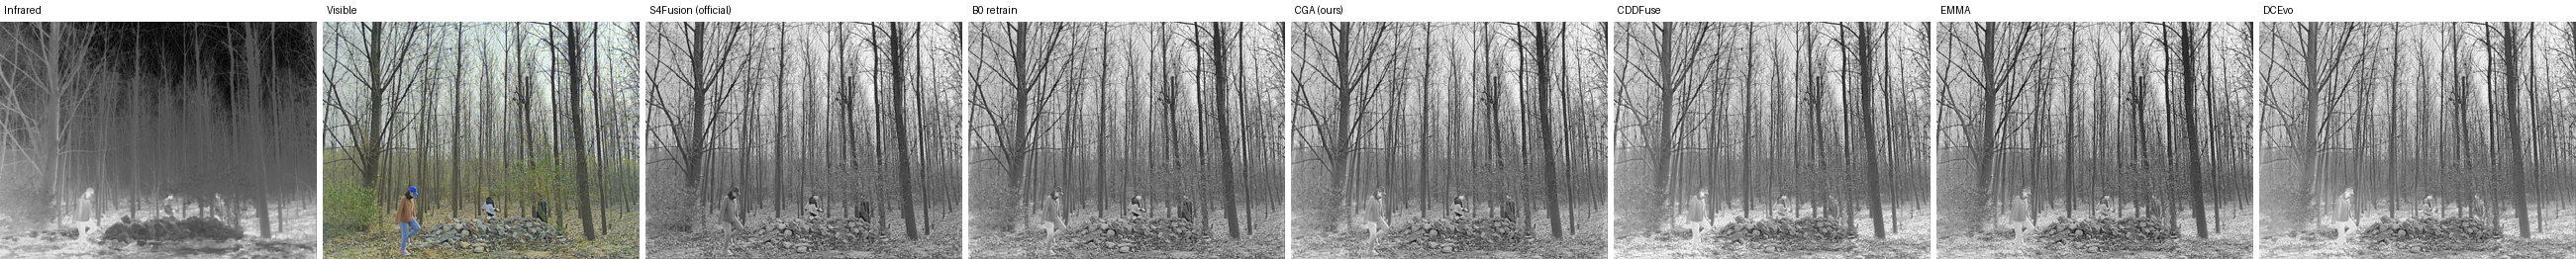
\includegraphics[width=\textwidth]{figs/qualitative_01406.png}\\[2pt]
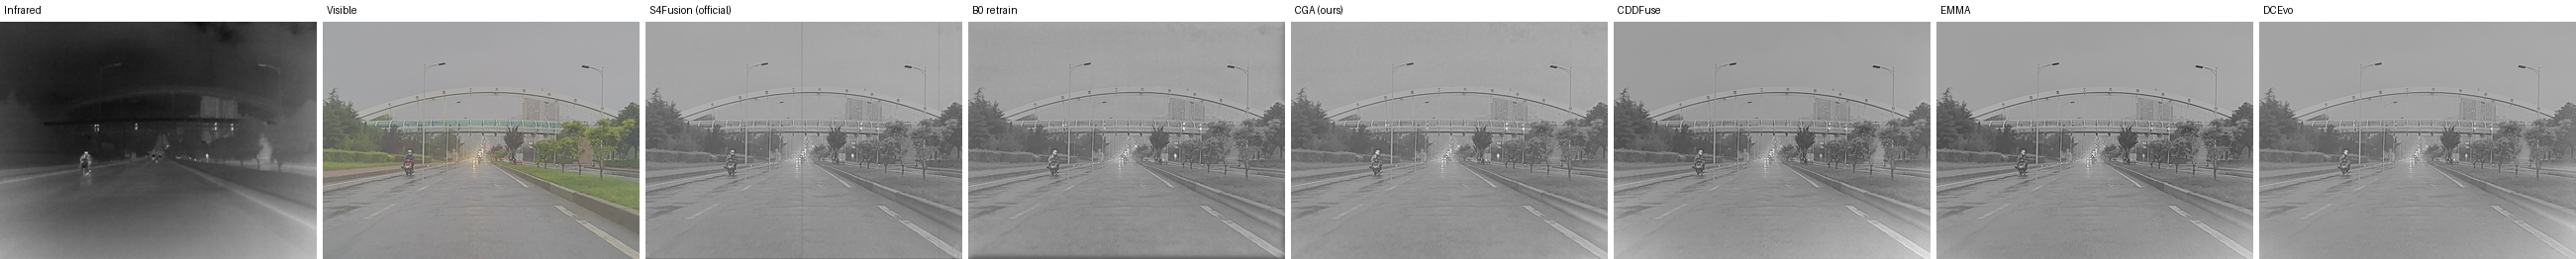
\includegraphics[width=\textwidth]{figs/qualitative_00097.png}
\caption{Qualitative comparison on two M3FD scenes (top: conflict-heavy scene 01406, drawn from the six highest-learning conflict samples of the frozen visualization record; bottom: regular scene 00097). All fused columns are produced by the unified evaluation protocol of Section~\ref{sec:exp:protocol}; no image was regenerated for this figure. The complete 300-image sets are released with the code.}
\label{fig:qualitative}
\end{figure*}

FusionMamba is the weakest row of the table across most metrics (EN 6.6103, SF 11.3349, AG 6.2939, QABF 0.2296). We record this honestly with its cause: its released weights are trained on KAIST, a pedestrian-surveillance domain that is out-of-distribution for the road-scene M3FD test set. This row is a domain-transfer observation, not a claim about the FusionMamba architecture; it does not affect the head-of-table conclusions.

\subsection{Cross-seed robustness}\label{sec:exp:seeds}

To rule out single-seed luck, the CGA-vs-B0 comparison is replicated over three training seeds (42, 123, 3407), each producing 300 fused image pairs per variant, pooled into 900 per-image paired deltas per metric. Table~\ref{tab:seeds} reports the pooled paired Wilcoxon test with Holm correction, using the image as the pairing unit.

\begin{table}[t]
\caption{Cross-seed robustness: pooled paired Wilcoxon (image = unit) with Holm correction, CGA $-$ B0 over 3 seeds $\times$ 300 images.}
\label{tab:seeds}%
\begin{tabular}{@{}lccc@{}}
\toprule
Metric & Pooled mean $\Delta$ (CGA$-$B0) & $p_{\mathrm{holm}}$ & Seed direction \\
\midrule
EN & $+0.0174$ & 1.31e$-$16 & 3+/0$-$ \\
MI & $+0.7066$ & 1.68e$-$146 & 3+/0$-$ \\
QABF & $+0.0113$ & 4.71e$-$137 & 3+/0$-$ \\
VIF & $+0.0073$ & 1.26e$-$97 & 3+/0$-$ \\
SF & $-0.0713$ & 1.09e$-$122 & 0+/3$-$ \\
AG & $-0.1295$ & 4.35e$-$147 & 0+/3$-$ \\
\botrule
\end{tabular}
\end{table}

The pattern is unambiguous in direction: the information- and fidelity-oriented metrics (EN, MI, QABF, VIF) all improve and the structural sharpness metrics (SF, AG) all degrade, with 100\% seed-direction consistency --- every one of the six metrics points the same way in all three seeds (3+/0$-$ or 0+/3$-$). The MI gain ($+0.7066$) is the largest absolute effect; the structural cost is discussed openly in Sections~\ref{sec:exp:verdicts} and~\ref{sec:exp:negative} rather than minimized. Per the pre-registered protocol, seed-level significance tests are intentionally omitted: with $n=3$ seeds the minimum achievable Wilcoxon $p$ is 0.25, so seed-level testing is uninformative, and direction consistency is reported descriptively instead. Because pooling the three seeds into a single $n=900$ test treats images from different seeds as independent units, we additionally re-ran the analysis per seed (each $n=300$, image as the pairing unit, Holm correction over the 18 seed$\times$metric tests): all 18 per-seed tests remain significant after correction (most conservative: EN on s42, $p_{\mathrm{Holm}}=0.0007$), the per-seed mean differences average digit-for-digit to the pooled values, and the direction pattern is identical --- so the pooled conclusions do not depend on the cross-seed independence assumption.

\subsection{Pre-registered hypothesis verdicts}\label{sec:exp:verdicts}

This section reports the verdicts on the pre-registered hypotheses, each against the judgment criterion fixed in the protocol before the experiment was run.

\paragraph{H1 --- feature-space $B/C/\Delta$ state modulation improves structural fusion --- falsified.}
Under the controlled same-budget ablation (same public S4Fusion starting weights, same budget, seed 42), the state-modulated variant significantly \emph{degraded} every structural metric relative to B0: SF $-0.0190$, AG $-0.0126$, QABF $-0.0005$, with Holm-corrected $p = 2.90\times10^{-44}$, $8.13\times10^{-40}$, and $5.63\times10^{-27}$ respectively. The protocol's pre-registered conclusion rule --- ``no structural metric with the state-modulated variant above B0 at Holm $p<0.05$'' --- was met by the negative direction: under this registered parameterization, the state-capacity-dilution account does not transfer to structural gains, and the paper's narrative pivots to image-space arbitration on the strength of this falsification, per the registered consequence of H1.

\paragraph{H5 --- CGA conflict-gated arbitration improves high-conflict detection --- primary criterion met on all three seeds.}
The pre-registered primary endpoint is high-conflict object recall on the full 300-image M3FD detection protocol, tested with an exact binomial (McNemar-style) test on recovered vs.\ lost objects. Table~\ref{tab:h5} shows that all three seeds reproduce the effect.

\begin{table}[t]
\caption{H5 primary endpoint: high-conflict object recall (vs.\ B0cmp\_full baseline) on M3FD full-300.}
\label{tab:h5}%
\begin{tabular}{@{}lccc@{}}
\toprule
Seed & High-conflict recall $\Delta$ & recovered / lost & $p$ (exact binomial) \\
\midrule
s42 & $+0.0194$ (0.4385$\to$0.4579) & 20/3 & 4.88e$-$04 \\
s123 & $+0.0159$ (0.4385$\to$0.4544) & 18/4 & 4.34e$-$03 \\
s3407 & $+0.0159$ (0.4385$\to$0.4544) & 18/4 & 4.34e$-$03 \\
\botrule
\end{tabular}
\end{table}

The identical s123/s3407 rows deserve an explicit note: a pixel-level comparison of the two seeds' fused outputs (60-image random sample) found zero byte-identical and zero pixel-identical images (median mean absolute difference $0.37$ over $0$--$255$; about 30\% of pixels differ by at least one grey level), so the seeds are genuinely independent runs whose detection statistics converge at the detector's quantization resolution --- 18 recovered and 4 lost objects happen to be the same counts --- rather than duplicated outputs.

Every seed shows a significant positive gain (all $p < 0.005$) with at least 14 more recovered than lost objects, satisfying the pre-registered H5 criterion (significant positive delta AND recovered$-$lost $\geq 3$) on all three seeds. The s123 and s3407 rows are numerically identical (18/4, the same counts; see the product-verification note below Table~\ref{tab:h5}).

\paragraph{Stricter pre-registered gates (C1/C2/C3) --- narrow-margin misses.}
Beyond the primary criterion, the protocol registered three stricter gates; none is passed in full.
\begin{itemize}
\item \textbf{gate-C1} (high-conflict recall $\Delta \geq +0.02$): all three seeds FAIL ($+0.0194$ / $+0.0159$ / $+0.0159$; the misses are narrow --- $0.0006$--$0.0041$ below the threshold).
\item \textbf{gate-C2} (mAP50 $\Delta \geq +0.01$ vs.\ B0cmp 0.7197): all three seeds FAIL (s42 $+0.0085 \to 0.7282$; s123 $+0.0028 \to 0.7225$; s3407 $+0.0035 \to 0.7232$).
\item \textbf{gate-C3} (SF/AG relative non-inferiority within $-1\%$, \texttt{struct\_noninferior.py}): s123 PASS (SF $-0.39\%$, AG $-0.60\%$) and s3407 PASS (SF $-0.21\%$, AG $-0.36\%$); s42 is the borderline exception --- SF $-0.85\%$ passes, AG $-1.00\%$ fails exactly at the threshold. Frozen wording: C3 passes on 2/3 seeds, with s42 an AG borderline exception.
\end{itemize}
The frozen verdict for the pre-registered grade table is therefore: between grades A and B, handled as B-leaning-A. The primary H5 criterion is satisfied on all three seeds (significant, direction-consistent high-conflict recall gains), but the three stricter gates are not met; the paper's wording for this residual gap is fixed throughout as ``statistically significant but below the stricter pre-registered gate thresholds'', and we never write that CGA ``passed the pre-registered gates''.

\subsection{Mechanism visualization}\label{sec:exp:vis}

The mechanism-level evidence verifies that CGA acts as designed rather than remaining inert. The global gate scale, which is zero-initialized so that loading the official checkpoint reproduces the baseline exactly, trains to saturation: $\tanh(\mathrm{gate\_scale}) = 0.9998$ on the CGA seed-42 checkpoint. This reading rules out the self-falsifying scenario in which the gate stays at zero and the measured gains would have to come from some other source; the arbitration path is genuinely open.

At the pixel level, the intervention is selective rather than global. On the six highest learned-conflict M3FD samples (01406, 01422, 01413, 01415, 01393, 01432), the mean absolute difference between CGA and B0 fused outputs is 0.0125--0.0170, while the peak difference-map value reaches 0.594. A small mean with a large peak is exactly the signature expected from a conflict-gated operator: most of the image (non-conflict regions) is left nearly untouched, while pixels in conflict regions are strongly re-assigned. Figures~\ref{fig:panel-a} and~\ref{fig:panel-b} show two of these panels --- source pair, learned conflict map, manual conflict map, CGA output, B0 output, and their difference map --- for the samples with the highest learned conflict (selected conflict panels; the full set of six is archived with the data release in \texttt{results/cga\_vis/}, one \texttt{*\_panel.png} and one \texttt{*\_cga.npz} per sample, and is given in the supplementary material).

\begin{figure}[t]
\centering
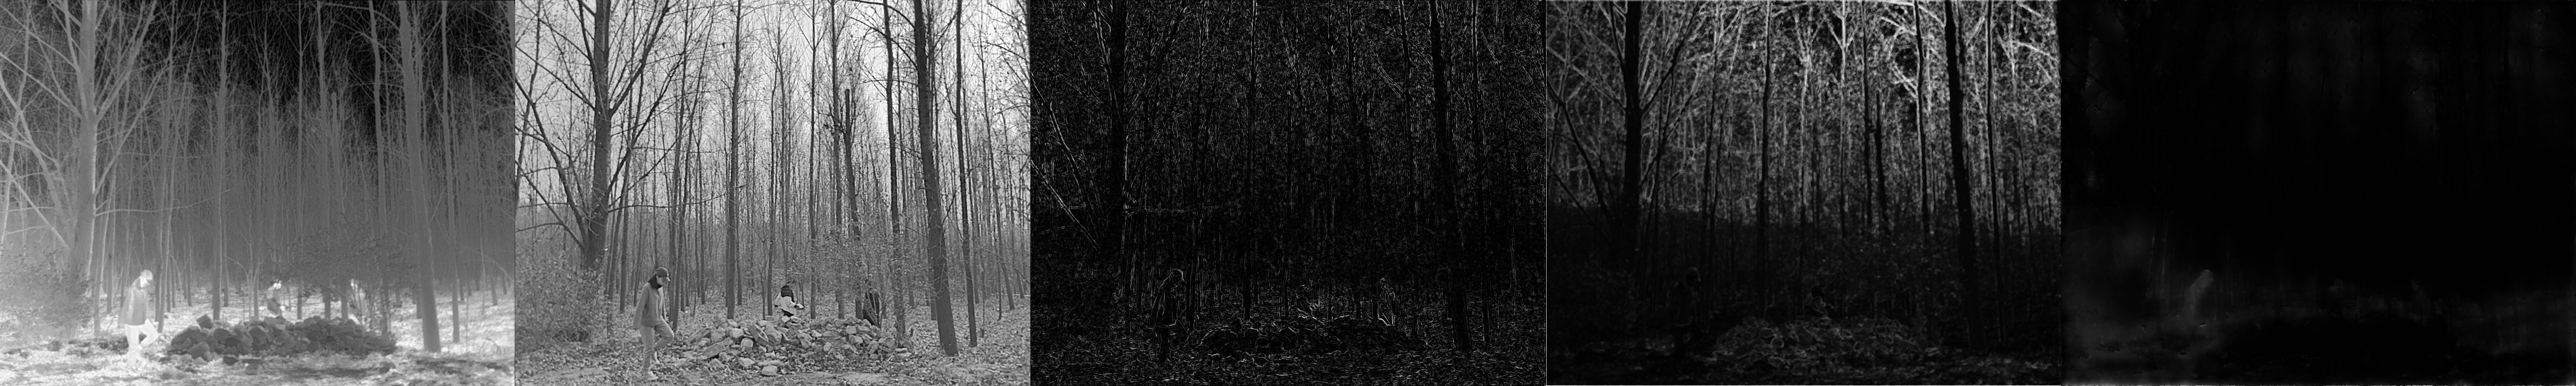
\includegraphics[width=0.92\textwidth]{figs/01406_panel.png}
\caption{Mechanism visualization on the highest learned-conflict M3FD sample 01406: source pair, learned conflict map, manual conflict map, CGA output, B0 output, and their difference map. The mean absolute CGA--B0 difference lies in 0.0125--0.0170 with a difference-map peak of 0.594: most of the image is untouched while conflict pixels are strongly re-assigned. Selected conflict panel; full set of six samples in the supplementary material.}
\label{fig:panel-a}
\end{figure}

\begin{figure}[t]
\centering
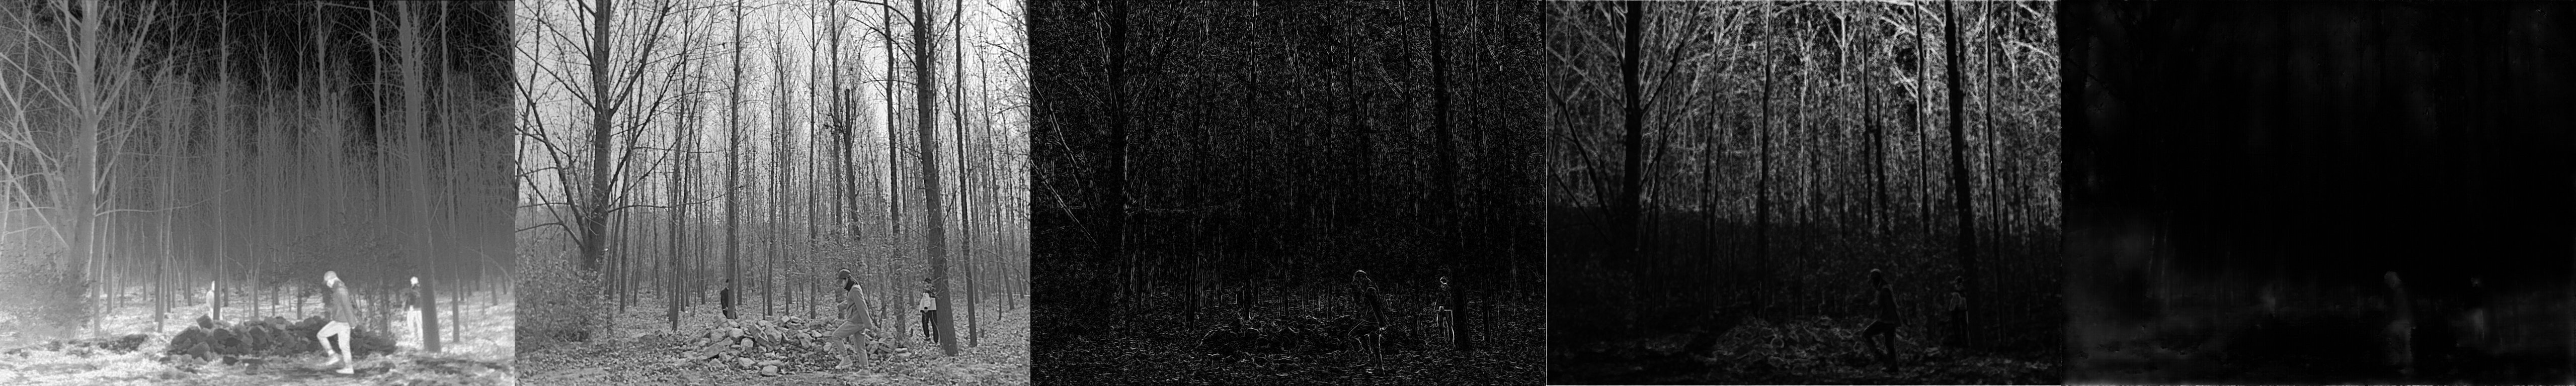
\includegraphics[width=0.92\textwidth]{figs/01422_panel.png}
\caption{Mechanism visualization on M3FD sample 01422, the second-highest learned-conflict sample: the CGA--B0 difference map concentrates in conflict regions where the learned conflict map is active, matching the selective-intervention signature of a conflict-gated operator (mean absolute difference 0.0125--0.0170, peak 0.594). Selected conflict panel; full set of six samples in the supplementary material.}
\label{fig:panel-b}
\end{figure}

The secondary cross-scale evidence supports the same proposition from the resolution axis. Under the multi-resolution stress protocol (120 paired images at five resolutions 289--769), the CGA variant shows significantly lower cross-scale drift than B0 at 4 of 5 resolutions, with drift-AUC reduced from 0.8088 to 0.7839 ($\Delta = -0.0249$, $p = 1.41\times10^{-5}$) --- including the highest resolution tested (769). This gain comes from the arbitration arm and is consistent with the reading that arbitration rather than averaging carries structure across scales.

\subsection{Color fidelity}\label{sec:exp:color}

Because CGA commits to a single modality's luminance in conflict regions, its effect on the chrominance channels deserves an explicit check (the protocol's color-fidelity audit). Color metrics are computed on the full 300-image set against the same-budget B0 comparison variant, with YCbCr reconstruction of the fused output. The outcome is mixed but interpretable, and we report it as such:
\begin{itemize}
\item \textbf{EOR} (edge-orientation retention, computed as the RGB-space edge-orientation agreement between the fused output and the source images) improves by $+0.0016$, significant (Wilcoxon $p = 8.7\times10^{-9}$).
\item \textbf{CIEDE2000} color difference decreases by $-0.229$ (i.e., closer to the visible reference), but this improvement is not significant at $p = 0.080$.
\item A descriptive RGB three-channel SSIM decreases by $-0.0093$ ($p = 1.25\times10^{-7}$), and Colorfulness decreases by $-0.0043$ ($p = 7.96\times10^{-12}$).
\end{itemize}
The mixed reading is coherent with the mechanism's known structural cost: the two small degradative deltas (RGB SSIM $-0.0093$, Colorfulness $-0.0043$) point in the same direction as the AG cost of hard commitment (Section~\ref{sec:exp:seeds}), while the edge-oriented metric improves significantly. In other words, color behavior is the chrominance-side echo of the same trade-off already disclosed in the luminance metrics --- not a new, unexplained failure mode. We describe the RGB metric as ``a descriptive three-channel SSIM on RGB'' rather than coining it as a named fusion metric, since it is used here only as a channel-wise fidelity descriptor.

\subsection{Negative results and failure analysis}\label{sec:exp:negative}

This paper's methodological stance is that pre-registered negative results are findings, and this section reports them without cosmetic repair.

\paragraph{H1 falsification (already reported in Section~\ref{sec:exp:verdicts}).}
The feature-space $B/C/\Delta$ modulation hypothesis was falsified under the controlled same-budget protocol: all structural metrics significantly degraded (SF $-0.0190$, AG $-0.0126$, QABF $-0.0005$; Holm $p \leq 5.63\times10^{-27}$). The registered consequence was executed: the ``mechanism-inside-the-SSM'' narrative was retired, not softened.

\paragraph{Distillation --- deterministic failure, reported as a negative result.}
The reliability-map distillation arm (teacher = trained CGA seed-42 model with depths 1,2,1; student with depths 1,1,1 and \texttt{-{}-use-cga}; output-L1 weight 1.0, feature SmoothL1 0.2, boundary-KL 0.5; 20 epochs, crop 128, seed 42) produced NaN validation loss in epoch 1 (train 6.959 / val NaN) and NaN train \emph{and} val losses for epochs 2 through 20; the best checkpoint was never saved (val = inf never updated), leaving only an unusable NaN-weights \texttt{\_last.pt}. Per the pre-registration discipline, we did not tune hyperparameters and did not rerun; the reliability-map component is reported as a first-attempt failure rather than a supported contribution. Two candidate explanations are on record for later work --- (a) the CGA commitment loss diverging in the distillation configuration (possibly the same phenomenon as the late-training NaNs below), and (b) an implementation issue in the boundary-KL/feature distillation path on a shallow student --- and neither is tested in this paper.

\paragraph{Late-training NaN instability in the CGA family.}
Across seeds, the CGA variants exhibit late-epoch validation NaN: seed 123 from epoch 12 and seed 3407 from epoch 13, while in the same replication queue the B0 family completes all 20 epochs without any NaN. The best checkpoints were saved before NaN onset in every case (s123 best at epoch 11, val 0.3090; s3407 best at epoch 12, val 0.3063), so all reported evaluation numbers come from valid pre-NaN checkpoints; the same instability type was previously observed in the seed-42 CGA run (best at epoch 26, val NaN from epoch 27). We record a mechanistic hypothesis --- the hard commitment loss (weight 10) plus the gate-LR path diverging late in training --- as an open item for future analysis; no hyperparameters were changed and no runs were repeated in this paper, per the same-budget discipline.

\subsection{Reproducibility}\label{sec:exp:repro}

\paragraph{Registered content controls of the conflict map (exploratory).}
The pre-registered protocol included two inference-time controls for the conflict map: a uniform all-ones map (commitment applied everywhere) and a spatially shuffled map (values preserved, positions destroyed). Complete per-image fusion outputs exist for all three conditions (300 images each, evaluated with five of the six metrics; VIF was not recorded by the evaluator build that produced them), and we report their paired comparison with three explicit caveats: the runs use the gate-LR variant checkpoint rather than the main-table checkpoint; the detector endpoint was not run on the control outputs; and the analysis is therefore exploratory. The comparison is unflattering to the learned map and we report it as-is: an all-ones conflict map \emph{increases} SF ($+2.41$), AG ($+0.65$), MI ($+2.35$) and, marginally, QABF ($+0.0084$) over the learned map (all Holm-corrected $p \leq 3.4\times10^{-42}$ except QABF at $3.02\times10^{-8}$), i.e., committing everywhere mechanically inflates gradient-energy and information metrics; and the shuffled map scores within a hair of the learned map (differences $-0.21$ to $+0.012$), i.e., the spatial arrangement of the conflict map contributes far less to fusion metrics than its presence. Two readings follow, both registered as interpretive: first, the fusion-quality metrics used throughout this field do not discriminate selective from indiscriminate commitment --- which is precisely why this paper's primary endpoints are mechanism-external (detector recall on a conflict subset defined before training, plus all-object mAP50), rather than fusion metrics; second, closing the control loop at the detector endpoint (uniform vs.\ learned conflict maps under the same detection protocol) remains future work that the released hooks make a single command away.

Every number in this paper can be regenerated from the frozen scripts in the repository. All training uses seeds 42/123/3407 via the standard seed switch; all statistical tables are auto-generated by the scripts named below, and every metric in this section traces to a per-image CSV produced by the unified evaluator \texttt{eval\_metrics.py}.

The main comparison table is produced by \texttt{aggregate\_sota.py}; the cross-seed table by \texttt{analyze\_seeds.py}; detection A/B endpoints are generated with \texttt{gen\_cga\_fused.py} followed by \texttt{arb\_detect\_full300.py} (run in the legacy environment); high-conflict statistics by \texttt{arb\_full300\_stats.py}; structural non-inferiority by \texttt{struct\_noninferior.py}. Mechanism visualization is produced by \texttt{cga\_visualize.py}; the seed training chain is orchestrated by \texttt{run\_seeds\_queue\_v2.sh} (with marker-file checkpointing) plus \texttt{run\_after\_seeds\_v2.sh} for the evaluation and distillation chain. The FusionMamba baseline is reproduced via \texttt{test\_m3fd.py} and \texttt{test\_m3fd\_pad32.py}, collected by \texttt{collect\_outputs.py}.

A reproducibility property specific to this design deserves emphasis: because the CGA gate is zero-initialized, the trained model can be loaded side-by-side with the official released S4Fusion weights, and setting the gate to zero recovers the baseline output exactly ($\tanh(0) = 0$). Any user of the released code can therefore verify on their own data that (i) the unmodified official weights are reproduced bit-exactly by the CGA-augmented model with the gate closed, and (ii) the deltas reported in this section come only from opening the gate.

%%=============================================================
%% §5 Discussion
%% Source: writing/06-discussion-conclusion.md §6
%%=============================================================
\section{Discussion}\label{sec:discussion}

This section reads the frozen evidence in three registers: what it supports, what it does not, and where the method sits. The paper's contribution is a verified mechanism with an honest evidence profile; conflating the registers would damage exactly that.

\subsection{What the evidence supports}\label{sec:discussion:supports}

The pre-registered question of this study was narrow by design: at pixels where the infrared and visible modalities disagree, does an explicit image-space per-pixel commitment toward the locally salient modality recover what blending loses? Three frozen observations support an affirmative answer at the level of mechanism.

First, the learned gate is genuinely engaged rather than latent. The zero-initialized global gate scale saturates after training at $\tanh(\mathrm{gate\_scale}) = 0.9998$, which excludes the self-falsification scenario in which the gate stays at zero and any measured difference originates elsewhere in the pipeline. Second, the intervention is selective rather than global: on the six highest-learning conflict samples, the mean absolute CGA--baseline difference lies in 0.0125--0.0170 with difference-map peaks up to 0.594, and the modifications concentrate in conflict regions --- exactly where the design intends them to act. Third, the direction of effect is stable across seeds. All six quality metrics are sign-consistent on 3/3 seeds (EN, MI, QABF, VIF positive; SF, AG negative), and the H5 primary criterion replicates on every seed: high-conflict recall gains of $+0.0194$, $+0.0159$ and $+0.0159$ (exact binomial $p = 4.88\times10^{-4}$, $4.34\times10^{-3}$ and $4.34\times10^{-3}$) with recovered-to-lost object ratios of 20:3, 18:4 and 18:4. Under the pre-registered decision rule --- $p < 0.05$ and recovered $-$ lost $\geq 3$ --- H5 is met on all three seeds; seed-level significance tests were omitted by the same pre-registration, since with $n = 3$ the minimum attainable $p$ is 0.25. The direction was first indicated by a training-free pre-check, in which committing toward the max-response modality in conflict regions recovers objects that blending loses; the learned gate confirms it under the registered criterion (cf.\ Introduction).

The profile of the quality metrics is coherent with this mechanism. Pooled per-image mean differences are positive for MI, QABF, VIF and EN, each with 3+/0$-$ seed-direction consistency; in the main comparison CGA attains the best QABF of the table (0.5449) and stays within $-0.0006$ of the best VIF (the official weights). One nuance deserves an explicit reading: relative to the official weights, the B0 retrain itself loses MI (4.3364 to 3.2078) while gaining QABF, and CGA recovers most of that MI loss (3.9345) on top of B0 --- so the CGA$-$B0 MI difference is partly a recovery of the retrain's MI cost rather than a gain over the official model, and we do not claim otherwise. Commitment at conflict pixels improves cross-modal information transfer and perceptual consistency rather than high-frequency gradient energy --- the two structural metrics that pay for it are treated in Section~\ref{sec:discussion:notsupport}. The multi-resolution stress axis points the same way: cross-scale drift-AUC falls from 0.8088 to 0.7839 ($p = 1.41\times10^{-5}$), with significantly lower drift on four of five resolutions. Committed outputs remain more consistent under rescaling --- supporting, though not by itself proving, the reading that arbitration rather than averaging carries structure across scales.

\subsection{What the evidence does not support}\label{sec:discussion:notsupport}

The freeze is equally explicit about the boundaries, and we report them in the same voice as the gains.

First, the magnitude of the primary detection gain is statistically significant but below the stricter pre-registered gate thresholds. Gate-C1 (high-conflict recall gain $\geq +0.02$) fails on all three seeds ($+0.0194$, $+0.0159$, $+0.0159$), and gate-C2 (mAP50 gain $\geq +0.01$ over the 0.7197 baseline) fails likewise ($+0.0085$, $+0.0028$, $+0.0035$). The frozen grade verdict retains the main narrative (mechanism significant, three-seed robust) while fixing the wording at ``below the stricter pre-registered gate thresholds''; at no point do we claim the stricter gates were passed.

Second, the structural cost is real, significant, and mechanism-inherent. SF and AG pool to $-0.0713$ and $-0.1295$ with 0+/3$-$ seed-direction consistency (Holm-corrected $p = 1.09\times10^{-122}$ and $4.35\times10^{-147}$), and RGB SSIM ($-0.0093$) and Colorfulness ($-0.0043$) move in the same direction. A mechanism-consistent reading is that committing to one modality removes the averaging that partially inflates gradient-energy metrics at boundaries; we report this as the expected price of arbitration, not training variance, while flagging the reading itself as interpretive. The pre-registered non-inferiority gate C3 passes on two of three seeds (s123: SF $-0.39\%$, AG $-0.60\%$; s3407: SF $-0.21\%$, AG $-0.36\%$) with s42 the borderline AG exception at exactly $-1.00\%$.

Third, the evidence mainline is single-dataset: every frozen number derives from M3FD, so no cross-dataset generalization claim is made. Fourth, the reliability-map distillation arm is a registered negative result --- validation NaN from the first epoch, no best checkpoint ever saved --- reported as a failure record, not rehabilitated.

\subsection{Positioning}\label{sec:discussion:positioning}

The comparison with the closest conflict-aware methods is defined on mechanism axes, not on gain magnitude. ARC3Fusion \cite{tian2026adaptive} coordinates consensus--complementarity--conflict in feature space through per-position three-branch Softmax weights that sum to one, and GatedFusion-Net \cite{brenner2026gatedfusion} learns per-pixel Sigmoid confidence masks applied additively; both are continuous, feature-space, soft coordinators. CGA differs on both axes at once: image space rather than feature space, and a hard commitment rather than a soft weight, triggered only where gradient-orientation or polarity conflict is detected. This positional distinction is independent of the gain magnitude --- a small gain weakens the practical-value claim, not the axis distinction --- and it is what survives the grade verdict intact.

The commitment philosophy itself has a long lineage. The classical select/choose fusion rules \cite{burt1993enhanced,zhang1999categorization,piella2003general} formalized choosing the salient source where sources disagree, and the learning-based multi-focus decision-map line \cite{ma2021endtoend} still makes per-pixel binary choices --- but driven by defocus within same-modality pairs. CGA inherits the commitment idea and moves it to cross-modal conflict: the trigger is inter-modal gradient conflict, the commitment is learned end-to-end, and it is applied through a zero-initialized gate that preserves official checkpoint compatibility at load time.

Finally, the positioning is deliberately that of a mechanism verification, not a comprehensive superiority claim. In the frozen main table EMMA leads SF and AG, and Diff-IF leads MI; CGA's leading metric is QABF, with VIF a statistical tie against the official weights. S4Fusion serves as the testbed because it is the representative open scan-and-blend selective state-space backbone whose public weights make the falsification controlled --- not because it is assumed to be the strongest backbone.

%%=============================================================
%% §6 Limitations
%% Source: writing/06-discussion-conclusion.md §7
%%=============================================================
\section{Limitations}\label{sec:limitations}

The following limitations are reported exactly as frozen; none is mitigated by post-hoc argument.

\begin{enumerate}
\item \textbf{Structural cost.} CGA trades high-frequency structure for arbitration: pooled SF/AG differences are $-0.0713$/$-0.1295$ with 0+/3$-$ seed consistency. The pre-registered C3 non-inferiority gate passes on 2/3 seeds; s42 is the AG borderline exception ($-1.00\%$, exactly at threshold).
\item \textbf{Narrow miss on the stricter gates.} C1 and C2 fail on all three seeds. The wording is fixed at ``statistically significant but below the stricter pre-registered gate thresholds'' and never claims the stricter gates were passed.
\item \textbf{Distillation failure and late-stage val NaN.} The reliability-map distillation arm never produced a usable checkpoint: validation NaN from epoch 1, NaN on all subsequent epochs, best never saved; only an unusable last checkpoint remains, and per pre-registration it was neither re-tuned nor re-run. Separately, CGA-line seeds exhibit late-stage val NaN (s123 from epoch 12, s3407 from epoch 13; best checkpoints 0.3090/0.3063 saved before onset), while the two B0-line seeds retrained in the same replication queue (s123, s3407) run all 20 epochs without NaN. The seed-42 CGA run whose best checkpoint feeds the main table selected its best at epoch 26 --- beyond the 20-epoch B0 schedule --- so the NaN-adjacent training length differs across arms; adopters who retrain the recipe on their own data face an unresolved divergence risk, and the frozen best-validation selection rule is the only safeguard in this round. A commit-loss divergence hypothesis is recorded and left for future work; this round does not act on it.
\item \textbf{Single-dataset mainline.} The frozen evidence is M3FD-only; out-of-distribution datasets were not part of this freeze round, and no generalization claim is made. The downstream-detection endpoint additionally uses a single fixed detector (the DCEvo detection branch) across all arms; within-arm comparisons are internally valid, but the absolute recall levels are detector-specific. A residual alternative explanation is therefore not fully closed: commitment shifts local contrast at conflict pixels, and part of the high-conflict recall gain could, in principle, reflect alignment of those shifts with this detector's preferences rather than improved fusion fidelity. The all-object mAP50 gains (positive on all three seeds, outside the conflict-subset definition) and the mechanism-external gate criteria are the evidence against this reading, but a second detector would be needed to close it definitively.
\item \textbf{Registration sensitivity.} The conflict signal $\kappa$ is computed from aligned source pairs; a 1--2 pixel misalignment can turn a shared edge into an apparent gradient-orientation conflict and trigger commitment toward one modality. The frozen experiments use the registered M3FD pairs, so no robustness claim is made for imperfectly registered inputs, and deployments with residual registration error should verify alignment upstream of the gate.
\item \textbf{Per-pixel independent gating.} The commitment decision is made independently at each pixel from local gradient conflict, with no spatial regularization on the commitment field. The observed concentration of modifications in conflict regions is an empirical property of the trained gate, not an architectural guarantee; spatially regularized commitment fields remain untested.
\item \textbf{Budget asymmetry between arms.} The CGA arm follows the registered 32-epoch extended schedule while the B0 baseline follows the unified 20-epoch schedule (Section~\ref{sec:methods}); no 32-epoch B0 control exists in the frozen record, so the CGA$-$B0 deltas bundle the gate, the commit-weighted loss, the gate learning rate, and the extended schedule. The asymmetry is not uniform across seeds: the best-validation checkpoints of the two NaN-affected CGA runs fall at epoch 11 (s123) and epoch 12 (s3407), both \emph{inside} the 20-epoch B0 budget, so for those two seeds the arms are matched in effective training length; only the seed-42 run, whose row feeds the main table, selected its best at epoch 26 and therefore exceeds the B0 schedule. A budget-matched 32-epoch B0 control for all three seeds remains the cleanest way to isolate the gate itself and is left to future work.
\end{enumerate}

%%=============================================================
%% §7 Conclusion
%% Source: writing/06-discussion-conclusion.md §8
%%=============================================================
\section{Conclusion}\label{sec:conclusion}

This study set out to locate the residual failure of scan-and-blend selective state-space fusion at modal boundaries. The controlled falsification returned a clear negative: feature-space modulation of the state dynamics, motivated by state-capacity dilution, significantly degrades rather than improves the structural metrics SF, AG and QABF under a same-budget protocol fine-tuned from identical public weights. Under this registered parameterization, the residual failure is not fixed inside the state; it is the absence of an arbitration decision where the modalities conflict, and on the representative testbed studied here the arbitration arm is what moves the pre-registered endpoints.

We introduced Conflict-Gated Arbitration as the corresponding mechanism: an image-space, conflict-triggered, per-pixel commitment toward the locally salient modality, carried by a zero-initialized gate that preserves the official checkpoint exactly at load time and saturates when trained. Across three seeds the primary pre-registered criterion replicates, the quality-metric directions are fully consistent, and the modifications concentrate where the modalities disagree.

The evidence boundary is reported with the same discipline: the detection gains are statistically significant but below the stricter pre-registered gate thresholds; significant SF/AG structural costs accompany them; the mainline is single-dataset; and the distillation arm is a registered failure. Within these boundaries, the contribution is a verified arbitration mechanism --- image-space per-pixel commitment at cross-modal conflict pixels --- together with the pre-registered, same-budget protocol that made both the falsification and the verification interpretable.

Whether spatially regularized commitment fields, cross-dataset validation, or a stabilized commit loss extend these gains remains open; we list them as questions, not promises.

%%=============================================================
%% Declarations
%%=============================================================
\backmatter

\bmhead{Data availability}The M3FD benchmark used in this study is publicly available from the TarDAL project \cite{liu2022tardal}. The per-image evaluation CSVs and mechanism-visualization panels supporting the conclusions of this article are included in the released code repository.

\bmhead{Code availability}The training, evaluation, and statistical-analysis scripts, together with the pre-registered protocol files, are released for full reproduction of every number reported in this paper.

\bmhead{Author contribution}Author Name: conceptualization, method design, experiments, analysis, writing.

\bmhead{Funding}[To be completed at submission: funding sources and grant numbers, or an explicit ``No funding was received'' statement.]

\bmhead{Competing interests}[To be completed at submission: declare any competing financial or non-financial interests, or an explicit ``The authors declare no competing interests.'']

\bmhead{Ethics approval and consent to participate / Consent for publication}Not applicable (no human participants or personal data; the M3FD benchmark is publicly released for research use).

\bmhead{Use of large language models and AI tools}In preparing this manuscript, the authors used AI-based assistance for three tasks: literature verification (cross-checking reference identities and the closest-neighbour characterizations cited in Section~\ref{sec:related}), statistical re-analysis scripting (the per-seed and paired-test computations of the frozen-data supplement), and language polishing. All experimental numbers were produced solely by the authors' frozen training and evaluation pipeline; every AI-assisted statement and number was checked against the frozen records by the authors, who take full responsibility for the content of the article.

%%=============================================================
%% Bibliography (sn-mathphys-num, numeric citations)
%%=============================================================
\bibliography{refs}

\end{document}
